%
% tiefe.tex -- Abhängigkeit von \varepsilon und \sigma von der Tiefe
%
% (c) 2021 Prof Dr Andreas Müller, OST Ostschweizer Fachhochschule
%
\documentclass[tikz]{standalone}
\usepackage{amsmath}
\usepackage{times}
\usepackage{txfonts}
\usepackage{pgfplots}
\usepackage{csvsimple}
\usetikzlibrary{arrows,intersections,math}
\begin{document}
\def\skala{1}
\begin{tikzpicture}[>=latex,thick,scale=\skala]

\def\s{1}
\newboolean{debug}
\setboolean{debug}{true}
\setboolean{debug}{false}

\node at (0,0) {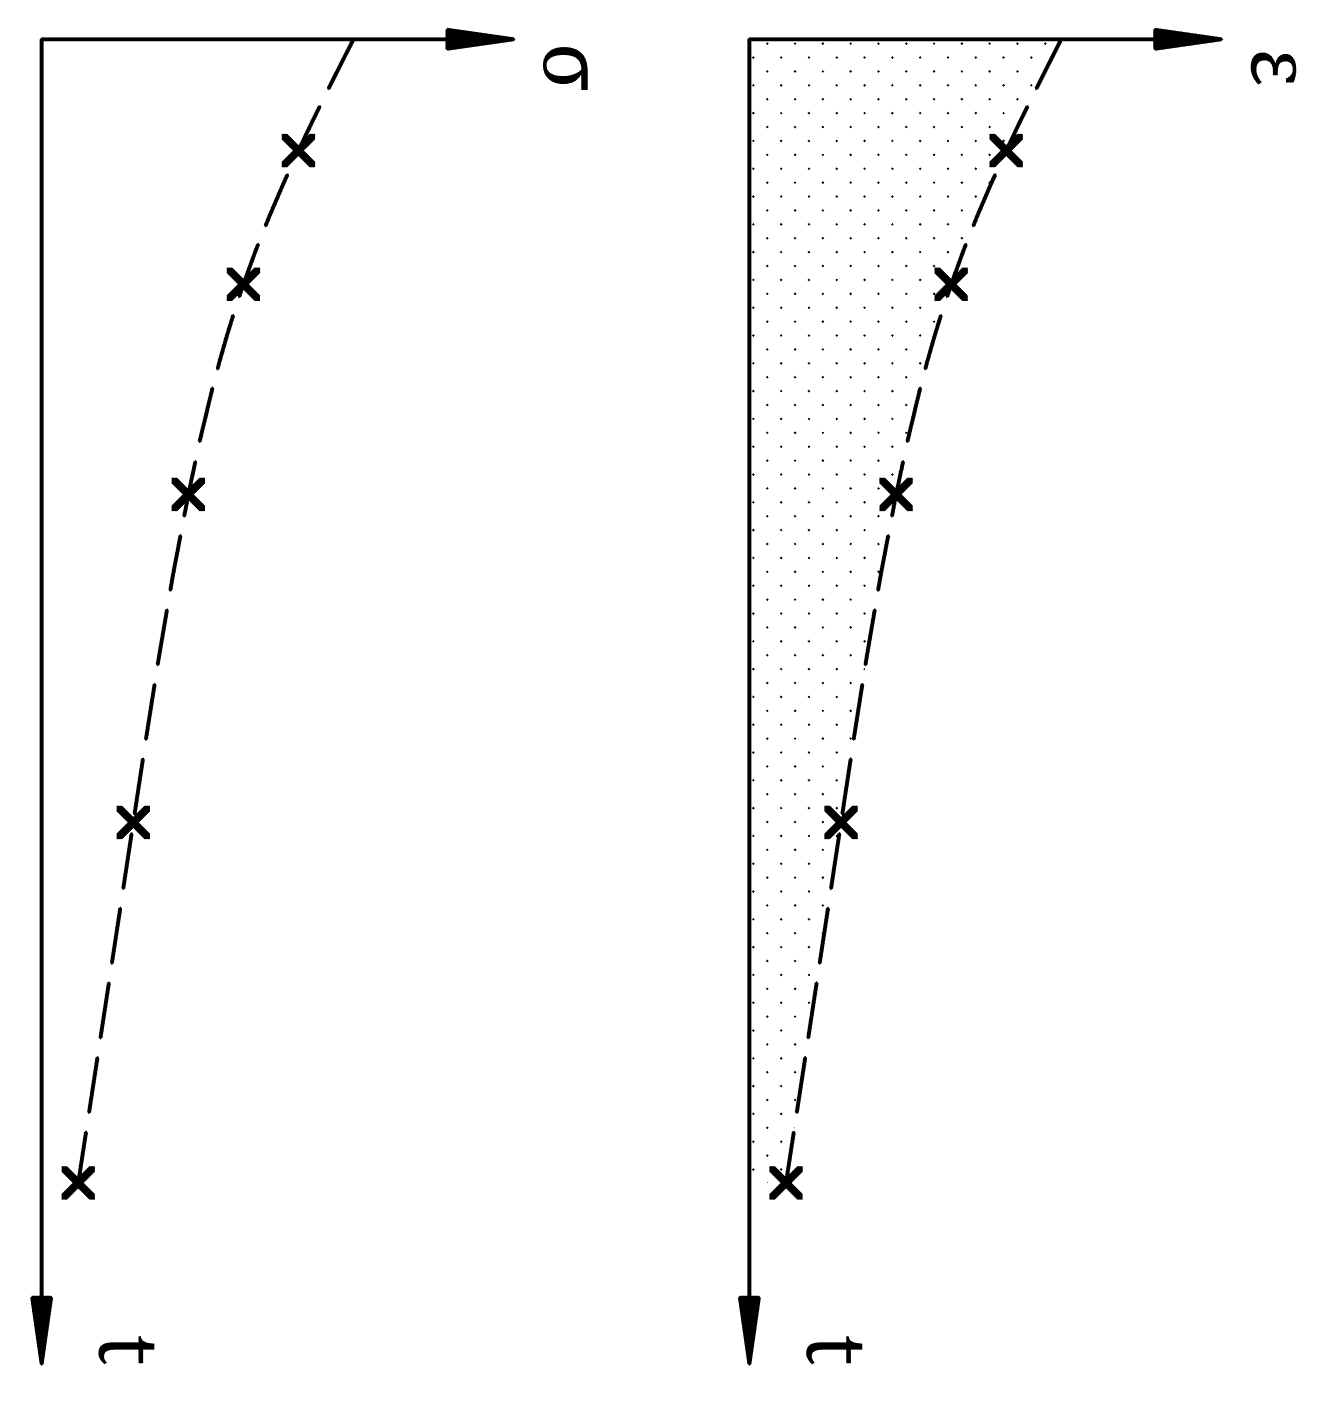
\includegraphics[width=6cm]{../Grafiken/Bild5.png}};
\def\beschriftung#1#2#3{
	\ifthenelse{\boolean{debug}}{
	\fill[color=red,opacity=0.2] ({(#1-0.22)*\s},{(#2-0.22)*\s})
		rectangle ({(#1+0.22)*\s},{(#2+0.22)*\s});
	}{
		\fill[color=white] ({(#1-0.22)*\s},{(#2-0.22)*\s})
			rectangle ({(#1+0.22)*\s},{(#2+0.22)*\s});
	}
	\node at ({#1*\s-0.1},{#2*\s}) {#3\strut};
}

\beschriftung{2.75}{2.9}{$\varepsilon$}
\beschriftung{-0.4}{2.9}{$\sigma$}

\beschriftung{-2.5}{-2.9}{$t$}
\beschriftung{0.67}{-2.9}{$t$}

\end{tikzpicture}
\end{document}

